    \begin{note}
        Ранее было доказанно, что $(1) \rightarrow (2), (2) \rightarrow (3), (1) \rightarrow (3).$ Рассмотрим более сложный переход: $(3) \rightarrow (1).$
    \end{note}
    \begin{theorem}
        Из леммы Кантора и леммы Архимеда следует аксиома непрерывности.
    \end{theorem}
    \begin{proof}
        Зафиксируем такие непустые множества $A, B \subset \R$, что $A$ расположенно левее $B.$ Разобьём доказательство на несколько шагов.
        
        \underline{Шаг 1.} Поскольку $A$ и $B$~---~непустые множества, зафиксируем произвольные $a_{0} \in A$ и $b_{0} \in B.$ Поскольку $A$ расположенно левее $B$, то $a_{0} \leq b_{0}.$

        \underline{Шаг 2.} Если $a_{0} = b_{0}$, то полагаем $c = a_{0} = b_{0}$ и завершаем доказательство. Действительно, если последовательнось $A$ <<левее>> последовательности $B$, то из $a \leq b \  \forall a \in A, \forall b \in B$ и $a_{0} \in A$ следует, что $\forall b \hookrightarrow b \geq a_{0} = c.$ Аналогично, $\forall a \hookrightarrow a \leq b_{0} = c.$

        \underline{Шаг 3.} Пусть теперь $a_{0} < b_{0}.$

        База индукции. Предположим, что при некотором $n \in \N$ мы построили такие отрезки, а при $n = 0$ мы это уже проверили. То есть
        $$ J^{0} = [a_{0}, b_{0}] \supset \ldots \supset J^{n} = [a_{n}, b_{n}],$$

        что справедливо неравенство

        $$\displaystyle l(J^{j}) = |a_{j} - b_{j}| \leq \frac{|a_{0} - b_{0}|}{2^{j}} \quad \forall j \in \{ 0, \dots, n \}.$$

        Кроме того,

        $$ J^{j} \cap A \neq \varnothing \  \text{ и  } J^{j} \    \cap B \neq \varnothing \quad \forall j \in \{ 0, \dots, n \}.$$

        Поделим отрезок $J^{n}$ на две равные части. Обозначим соответствующие отрезки символами $I^{n+1}_{1}, I^{n+1}_{2}$ в порядке следования (слева направо). Возможны 2 случая.

        В первом случае найдётся такой индекс $k^{*} \in \{ 1, 2\}$, что

        $$ I^{n + 1}_{k^{*}} \cap A \neq \varnothing \quad \text{и} \quad I^{n + 1}_{k^{*}} \cap B \neq \varnothing .$$

        Тогда положим

        $$ J^{n + 1} := I^{n + 1}_{k^{*}} .$$

        Во втором случае $I^{n + 1}_{1}$ имеет непустое пересечение только с $A$, а $I^{n + 1}_{2}$ имеет непустое пересечение только с $B.$ Тогда положим $c_{n} := \frac{a_{n} + b_{n}}{2} .$ Мы утверждаем, что

        $$ a < c_{n} < b \quad \forall a \in A, \forall b \in B.$$

        Действительно, поскольку $I^{n + 1}_{1} \cap A \neq \varnothing$ и $A$ расположенно левее $B$, то заведомо \newline $B \subset [a_{n}, +\infty).$

        С другой стороны, $I^{n + 1}_{1} \cap B \neq \varnothing$, откуда следует, что

        $$\displaystyle B \subset [a_{n}, +\infty) \  \backslash \  [c_{n}, b_{n}] = \bigg( \frac{a_{n} + b_{n}}{2}, +\infty \bigg) .$$

        Аналогично доказывается, что $A \subset (-\infty, \frac{a_{n} + b_{n}}{2}).$ Таким образом, выполнено условие $a < c_{n} < b.$ В частности, число $c_{n}$ разделяет множества $A$ и $B.$

        \underline{Шаг 4.} В итоге, возможны два случая. В первом случае (назовём его \textit{С1}), существует число $n_{0} \in \N$, для которого левая половина отрезка $[a_{n_{0}}, b_{n_{0}}]$ имеет непустое пересечение только с $A$, а правая половина имеет непустое пересечение только с $B.$

        Во втором случае (назовём его \textit{С2}), мы получим бесконечную последовательность отрезков $\{ J^{n} \}^{\infty}_{n = 0}$, для которой выполнены следующие свойства:

        (P1) $$J^{n + 1} \subset J^{n} \quad \forall n \in \N_{0};$$

        (P2) $$ J^{n} \cap A \neq \varnothing \  \text{ и } \   J^{n} \cap B \neq \varnothing \quad \forall n \in \N;$$

        (P3) $$\displaystyle l(J^{n}) = \frac{|a_{0} - b_{0}|}{2^{n}} \leq \frac{|a_{0} - b_{0}|}{n} \quad \forall n \in \N. \qquad (1)$$

        \underline{Шаг 5.} В случае (\textit{C1}) мы полагаем $c := \frac{a_{n_{0}} + b_{n_{0}}}{2}$ и завершаем построение, поскольку $c$ разделяет $A$ и $B$.

        \underline{Шаг 6.} В случае (\textit{C2}) заметим, что в силу (P1) и (P3) последовательность $\{ J^{n} \}^{\infty}_{n = 0}$ является стягивающейся последовательностью вложенных отрезков. Имея в виду теорему о существовании и единственности общей точки для стягивающейся последовательности вложенных отрезков, положим

        $$\displaystyle c := \bigcap_{n = 0}^{\infty} J^{n}.  \qquad\qquad (2)$$

        Покажем, что в этом случае $c$ разделяет $A$ и $B$. Рассуждая методом от противного, предположим, что найдётся $a^{*} \in A$ такое, что $a^{*} > c.$ В силу леммы Архимеда и (1) получим, что найдётся $n^{*} \in \N$ такое, что

        $$ l(J^{n^{*}}) < |c - a^{*}| \qquad (3)$$

        \newpage
        Но тогда, имеем

        $$ x < a^{*} \  \forall x \in J^{n^{*}}. \qquad (4)$$

        Действительно, в противном случае мы имели бы $|c-x| \geq |c - a^{*}|$ для некоторой точки $x \in J^{n^{*}}$, что в комбинации с (2) приводит к неравенству $l(J^{n^{*}}) \geq |c-a^{*}|$, которое противоречит (3).

        В силу (P2) отрезок $J^{n^{*}}$ имеет непустое пересечение с $B$, а значит существует $b^{*} \in J^{n^{*}} \cap B.$ Учитывая (4) получаем, что

        $$ \exists b^{*} \in B: \quad b^{*} < a^{*} \in A.$$

        Это противоречит тому, что множество $A$ расположено левее множесва $B$. Наше противоречие возникло от предположения, что существует точка $a^{*} \in A$, удовлетворяющая неравенству $a^{*} > c$. Значит наше предположение было неверно. Поэтому

        $$ a \leq c \quad \forall a \in A.$$

        Аналогично доказывается, что

        $$ c \leq b \quad \forall b \in B.$$

        Комбинируя последние два вывода, получаем аксиому непрерывности.
    \end{proof}
    \subsection{Счётные и несчётные множества}
    \begin{definition}
        Отображение $f$: $X \mapsto Y$ называется \textit{биекцией} $X$ на $Y$, если оно и инъекция, и сюръекция $\Leftrightarrow$ оно обратимо.
    \end{definition}
    \begin{definition}
        Множество $X$ называется \textit{конечным}, если $\exists N \in \N$ и биекция $X$ на $\{1, \dots, N \}.$ В противном случае множество называется \textit{бесконечным}.
    \end{definition}
    \begin{definition}
        Будем говорить, что \textit{множества $X \text{и } Y$ равномощны}, если существует биекция $X$ на $Y.$
    \end{definition}
    \begin{definition}
        Будем говорить, что \textit{мощность множества $Y$ не меньше мощности множества $X$}, если существует множество $Y^{'} \subset Y$ такое, что $X$ и $Y^{'}$ равномощны.
    \end{definition}
    \begin{definition}
        Множество $X$ называется \textit{счётным}, если $X$ равномощно $\N.$
    \end{definition}
    \begin{definition}
        Множество $X$ называется \textit{несчётным}, если $X$ бесконечно и неравномощно $\N.$
    \end{definition}
    \begin{theorem}
        $\Q$~---~счётно.
    \end{theorem}
    \begin{proof}
        Построим бесконечную таблицу. Где по горизонтали отложим целые числа, по вектикали~---~натуральные, а в клетках~---~их частное.
    \begin{center}
\begin{tabular}{|c||c|c|c|c|c|c|c|c|}
\hline
\textbf{$\N \backslash \Z$} & \textbf{0} & \textbf{1} & \textbf{-1} & \textbf{2} & \textbf{-2} & \textbf{3} & \textbf{-3} & \textbf{\dots} \\ \hline \hline
\textbf{1}  & 0/1        & 1/1        & -1/1        & 2/1        & -2/1        & 3/1        & -3/1        & $\dots$          \\ \hline
\textbf{2}  & 0/2        & 1/2        & -1/2        & 2/2        & -2/2        & 3/2        & -3/2        & $\dots$          \\ \hline
\textbf{3}  & 0/3        & 1/3        & -1/3        & 2/3        & -2/3        & 3/3        & -3/3        & $\dots$          \\ \hline
\textbf{4}  & 0/4        & 1/4        & -1/4        & 2/4        & -2/4        & 3/4        & -3/4        & $\dots$          \\ \hline
\textbf{$\vdots$}  & $\vdots$          & $\vdots$          & $\vdots$           & $\vdots$          & $\vdots$           & $\vdots$          & $\vdots$           & $\ddots$         \\ \hline
\end{tabular}
\end{center}
Будем двигаться по <<змейке>> из левого верхнего угла (0/1), нумеруя все попадающиеся рациональные числа, пропуская при этом те, которые встречались ранее. 

\begin{center}
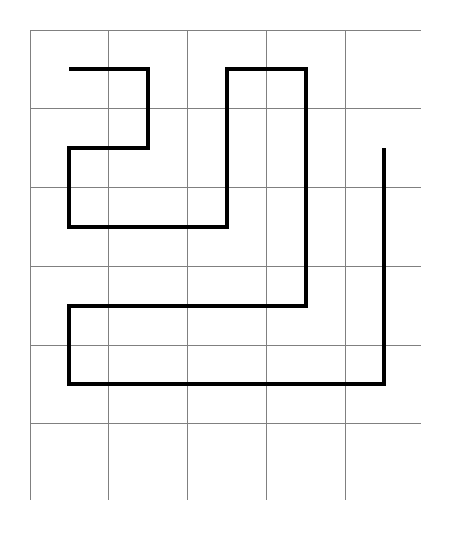
\begin{tikzpicture}[>=stealth]
    % Рисуем сетку
    \draw[help lines, step=1][gray]
    (-2,-3) grid (3,3);
    \draw[line width =.06cm, white] (3, 3) -- (3, -3);
    \draw[line width =.06cm, white] (-2, -3) -- (3, -3);
   \draw[line width =.05cm]  (-1.5, 2.5) --  (-0.5, 2.5) -- (-0.5, 1.5) -- (-1.5, 1.5) -- (-1.5, 0.5) -- (0.5, 0.5) -- (0.5, 2.5) -- (1.5, 2.5) -- (1.5, -0.5) --(-1.5, -0.5)-- (-1.5, -1.5) -- (2.5, -1.5) -- (2.5, 1.5);
    \end{tikzpicture}
\end{center}

Таким способом мы занумеруем все рациональные числа, засчёт чего получим инъекцию $\N \mapsto \Q.$

Так как для любого рационального числа найдётся <<квадрат>>, в которое это число попадает, то <<змейка>> через него пройдёт $\Rightarrow$ получаем сюръекцию.

Итого это инъекция и сюръекция, получаем биекцию $\Rightarrow \N \leftrightarrow \Q$ ($\N$ равномощно $\Q$.)
    \end{proof}

    \begin{theorem}
        $\R$~---~\textit{несчётно}.
    \end{theorem}
    \begin{proof}
        $\R$~---~бесконечно, поскольку содержит $\N$. Покажем, что $\R \nleftrightarrow \N.$

        Предположим противное, то есть существует биекция $\N \leftrightarrow \R.$ То есть все точки оказались пронумерованы натуральными числами. Тогда рассмотрим точку $x_{1}$ и отрезок $J^{1}$, не содержащий её. Внутри $J^{1}$ найдём отрезок $J^{2}$, не содержащий $x_{2}$, и заметим, что он не содержит и $x_{1}$. Продолжая по индукции, построим последовательность $J^{1} \supset J^{2} \supset \ldots \supset J^{k} \supset \dots$ со следующим свойством:

        $$ \forall k \in \N \quad x_{k} \notin J^{k}$$

        Следовательно $\{ x_{1}, x_{2}, \dots, x_{k} \} \cap J^{k} = \varnothing \quad \forall k \in \N.$

        По лемме Кантора существует точка $c$~---~пересечение последовательности вложенных отрезков ($c \in J^{k} \  \forall k \in \N$) $\Rightarrow c \neq x_{k} \   \forall k \in \N \Rightarrow$ мы нашли точку $c$, которой не присвоен никакой номер $\Rightarrow$ противоречие с тем, что все числа занумерованы.
    \end{proof}

    \newpage
    
\section{Предел числовой последовательности}

\subsection{Определение предела последовательности}
\begin{definition}
    \textit{Последовательностью} будет называть отображение $x$: $\N \mapsto \R.$
\end{definition}
\begin{note}
    При этом $x(n) \equiv x_{n} \quad \forall n \in \N.$
    
    Элементом последовательности называется пара $(n, x_{n}).$ При этом числа $x_{n}$ называются значениями элементов последовательности.
    
    Вся последовательность обозначается $\{ x_{n} \} \equiv \{ x_{n} \}^{\infty}_{n = 1}$
\end{note}
\begin{definition}
    $\Hat{\R} := \overline{\R} \cup \{ \infty \} = \R \cup \{ -\infty \} \cup \{ +\infty \} \cup \{ \infty \}$~---~\textit{расширенная числовая прямая}.
\end{definition}
\begin{note}
    Притом $\infty \neq \{ -\infty \}$, $\infty \neq \{ +\infty \}$.
\end{note}
\begin{definition}
    (\textit{Эпсилон окрестность из} $\Hat{\R}$) пусть $\epsilon > 0$, тогда 
    
    $$\text{если } a \in \R, \text{то } U_{\epsilon}(a) = (a - \epsilon, \ a + \epsilon)$$

    $$\text{если } a = +\infty, \text{то } U_{\epsilon}(a) = \bigg( \frac{1}{\epsilon}, \  + \infty \bigg)$$

    $$\text{если } a = -\infty, \text{то } U_{\epsilon}(a) = \bigg( -\infty, \  \frac{1}{\epsilon} \bigg)$$

    $$\text{если } a = \infty, \text{то } U_{\epsilon}(a) = U_{\epsilon}(-\infty) \cup U_{\epsilon}(+\infty)$$
\end{definition}
\begin{definition}
    Пусть $\{ x_{n} \}$~---~числовая последовательность. Будем говорить, что элемент $a \in \Hat{\R}$ является \textit{пределом последовательности} $\{ x_{n} \}$ и писать $\lim\limits_{n\to \infty} x_{n}=a \Leftrightarrow \newline x_{n} \rightarrow a, n \rightarrow \infty$, если выполнено следующее:

    $$ \forall \epsilon > 0 \  \exists N(\epsilon) \in \N: \  \forall n \geq N \hookrightarrow x_{n} \in U_{\epsilon}(a)$$
\end{definition}
\begin{note}
    То есть начиная с какого-то номера ($N$) все элементы последовательности с большим номером ($n \geq N$) попадут в заданный интервал ($U_{\epsilon}(a)$). Необязательно искать именно минимальный номер $N$.
\end{note}
\begin{example}
    Рассмотрим последовательность $\{ x_{n} \} = \{ \frac{1}{n} \}.$
    
    Покажем, что $\lim\limits_{n\to \infty} \frac{1}{n} = 0.$

    $$\forall \epsilon > 0 \  \exists N(\epsilon) = \bigg[ \frac{1}{\epsilon} \bigg] + 1: \forall n \geq N(\epsilon) \hookrightarrow \frac{1}{n} \leq \frac{1}{N(\epsilon)} \leq \frac{1}{[ \frac{1}{\epsilon}] + 1} \leq \frac{1}{\epsilon} = \epsilon.$$
     
\end{example}